%%%%%%%%%%%%%%%%%%%%%%%%%%%%%%%%%%%%%%%%%%%%%%%%
% COPYRIGHT: (C) 2012-2015 FAU FabLab and others
% Bearbeitungen ab 2015-02-20 fallen unter CC-BY-SA 3.0
% Sobald alle Mitautoren zugestimmt haben, steht die komplette Datei unter CC-BY-SA 3.0. Bis dahin ist der Lizenzstatus aller alten Bestandteile ungeklärt.
%%%%%%%%%%%%%%%%%%%%%%%%%%%%%%%%%%%%%%%%%%%%%%%%


\newcommand{\basedir}{fablab-document}
\documentclass{\basedir/fablab-document}

% \usepackage{fancybox} %ovale Boxen für Knöpfe - nicht mehr benötigt
\usepackage{amssymb} % Symbole für Knöpfe
\usepackage{subfigure,caption}
\usepackage{eurosym}
\usepackage{tabularx} % Tabellen mit bestimmtem Breitenverhältnis der Spalten
\usepackage{wrapfig} % Textumlauf um Bilder
\usepackage{enumitem}
\usepackage{listings}
\renewcommand{\texteuro}{\euro}
\newcommand*\circled[3]{\node[shape=circle,draw,inner sep=2pt,fill=green] at ({#1},{#2}) (char) {#3}}
\newcommand*\tikzcircled[1]{\tikz[baseline=(char.base)]{
            \node[shape=circle,draw,inner sep=2pt,fill=green] (char) {#1};}}

% \linespread{1.2}

\fancyhead[C]{\todo{unfertig!}}
\date{2013}
\author{kontakt@fablab.fau.de}
\title{Einweisung Mini-Fräse Roland iModela}

\begin{document}
~
\section{Regeln und Hinweise}
\begin{itemize}
\item Anleitung exakt beachten, wenn du nicht ganz genau weißt was du
tust.
\item Verletzungsgefahr am Fräser!
\item Fräskopf nicht von Hand bewegen, sondern über die PC-Software. (Siehe \ref{verfahren})
\item Nur geeignete Materialien verwenden. Kein leitfähiges Material! Im Zweifelsfall frage einen Betreuer.
\item Maschine nach jeder Benutzung reinigen!
\item Job erst starten, wenn alle Abdeckungen geschlossen sind. Diese müssen geschlossen bleiben, solange sich die Spindel dreht.
\item weitere Informationen in der Bedienungsanleitung unter\\ \texttt{Dateifreigabe/1\_fablab/iModela/iModela User Manual}
\end{itemize}
\section{Datenaufbereitung}
Die Fräsdaten für die iModela können entweder als 2D-Graphik vorliegen, die dann eine bestimmte Tiefe in das Material gefräst werden (2,5D) oder als dreidimensionales Objekt (3D). Falls die Daten schon fertig vorliegen akzeptiert die Software für 2,5D \emph{.eps} und \emph{.ai}-Dateien, die Software für 3D \emph{.stl} \todo{...}
\subsection{2,5D}
\begin{itemize}
\item \todo{...}
\end{itemize}

\subsection{3D}
\todo{...}

\section{Maschine vorbereiten}
\subsection{Maschine ein- und ausschalten}
\begin{itemize}
	\item \emph{iModela Controller} starten \todo{Bild}
	\item Maschine am Power-Knopf oben einschalten \todo{Bild}
	\item ausschalten in umgekehrter Reihenfolge
\end{itemize}

Falls sich keine Verbindung aufbauen lässt:
\begin{itemize}
	\item USB-Verbindung überprüfen
	\item Netzstecker ziehen und nochmals versuchen
\end{itemize}

\subsection{Maschine aufklappen}
\label{aufklappen}
\begin{itemize}
	\item Front- und Rückverkleidung aufklappen
	\item Seitenverkleidung aufklappen
	\item Die grünen Haken nach vorne lösen
	\item Haupteinheit vorsichtig nach hinten drücken
\end{itemize}
\begin{center}
	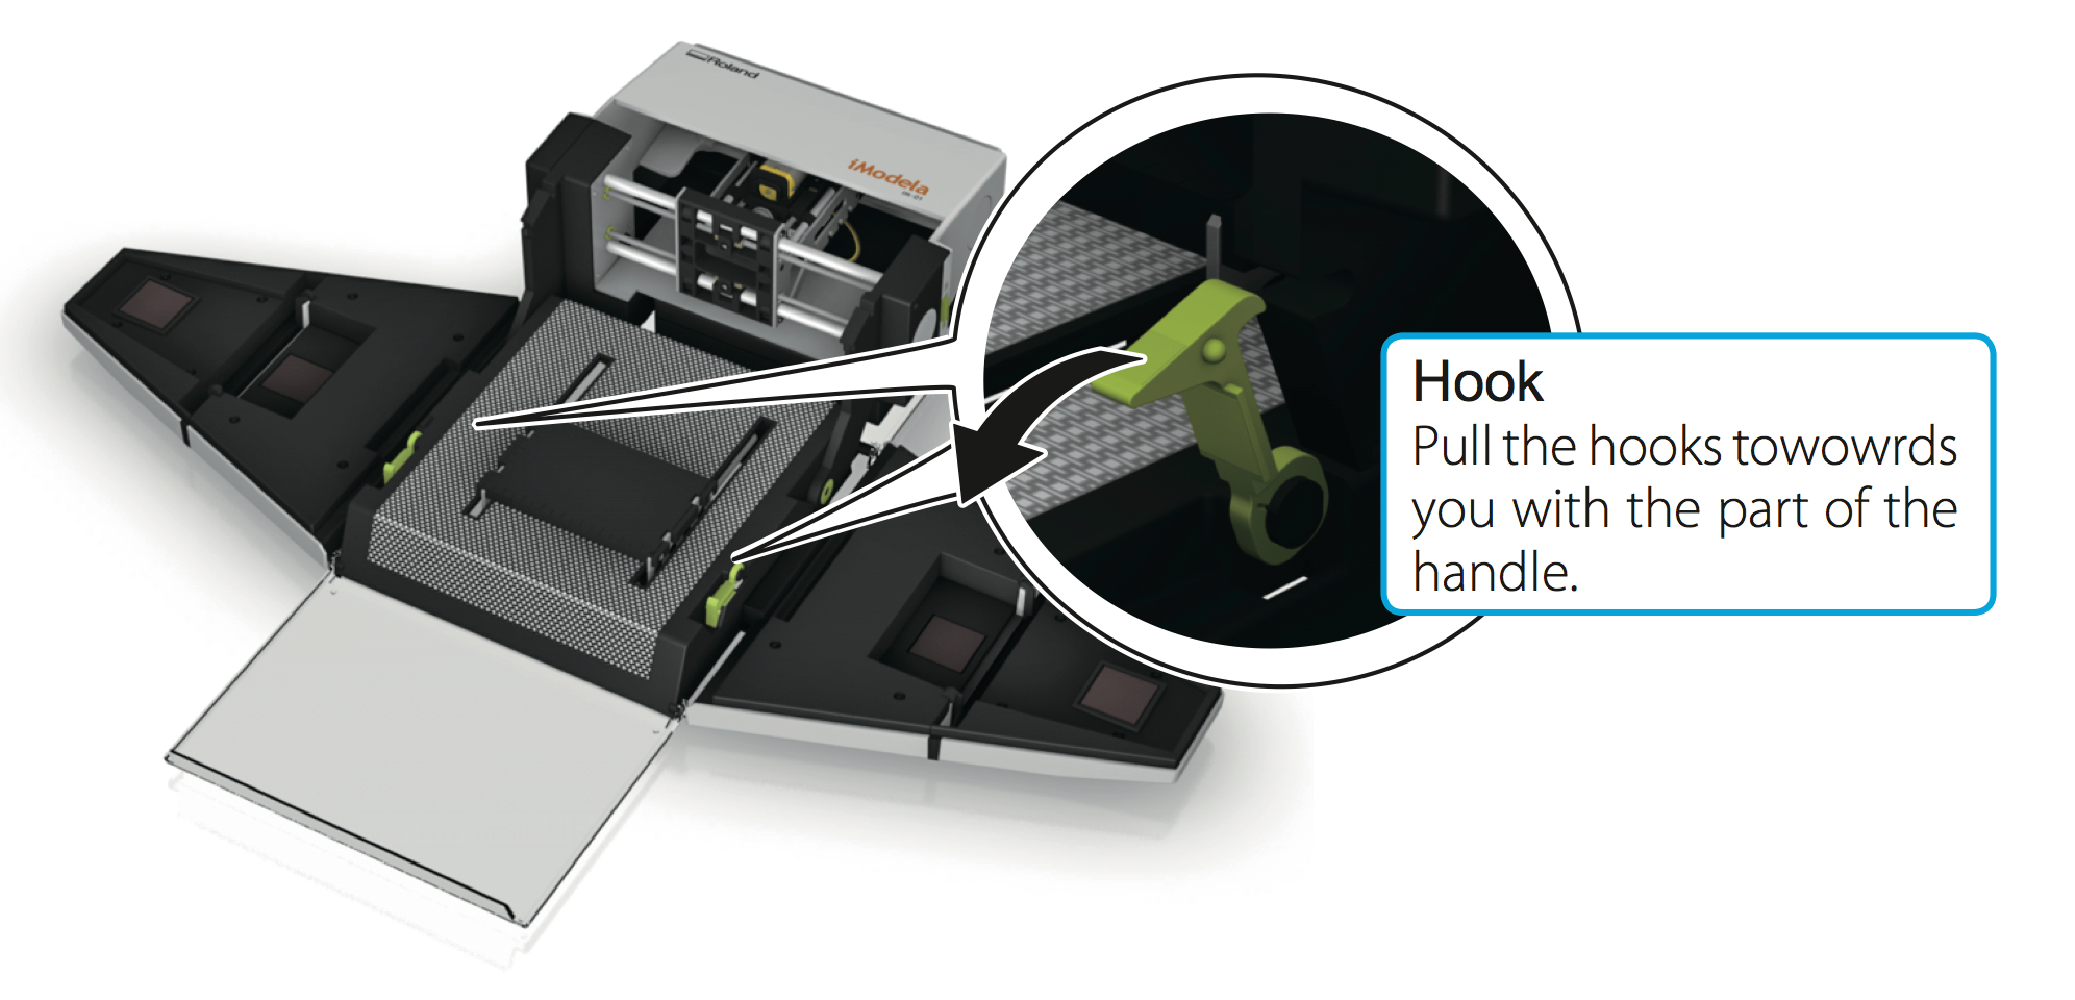
\includegraphics[width=0.8\textwidth]{img/aufklappen}
\end{center}

\subsection{Manuelles Verfahren}
\label{verfahren}
\begin{center}
\begin{tikzpicture}
    \node[anchor=south west,inner sep=0] at (0,0) {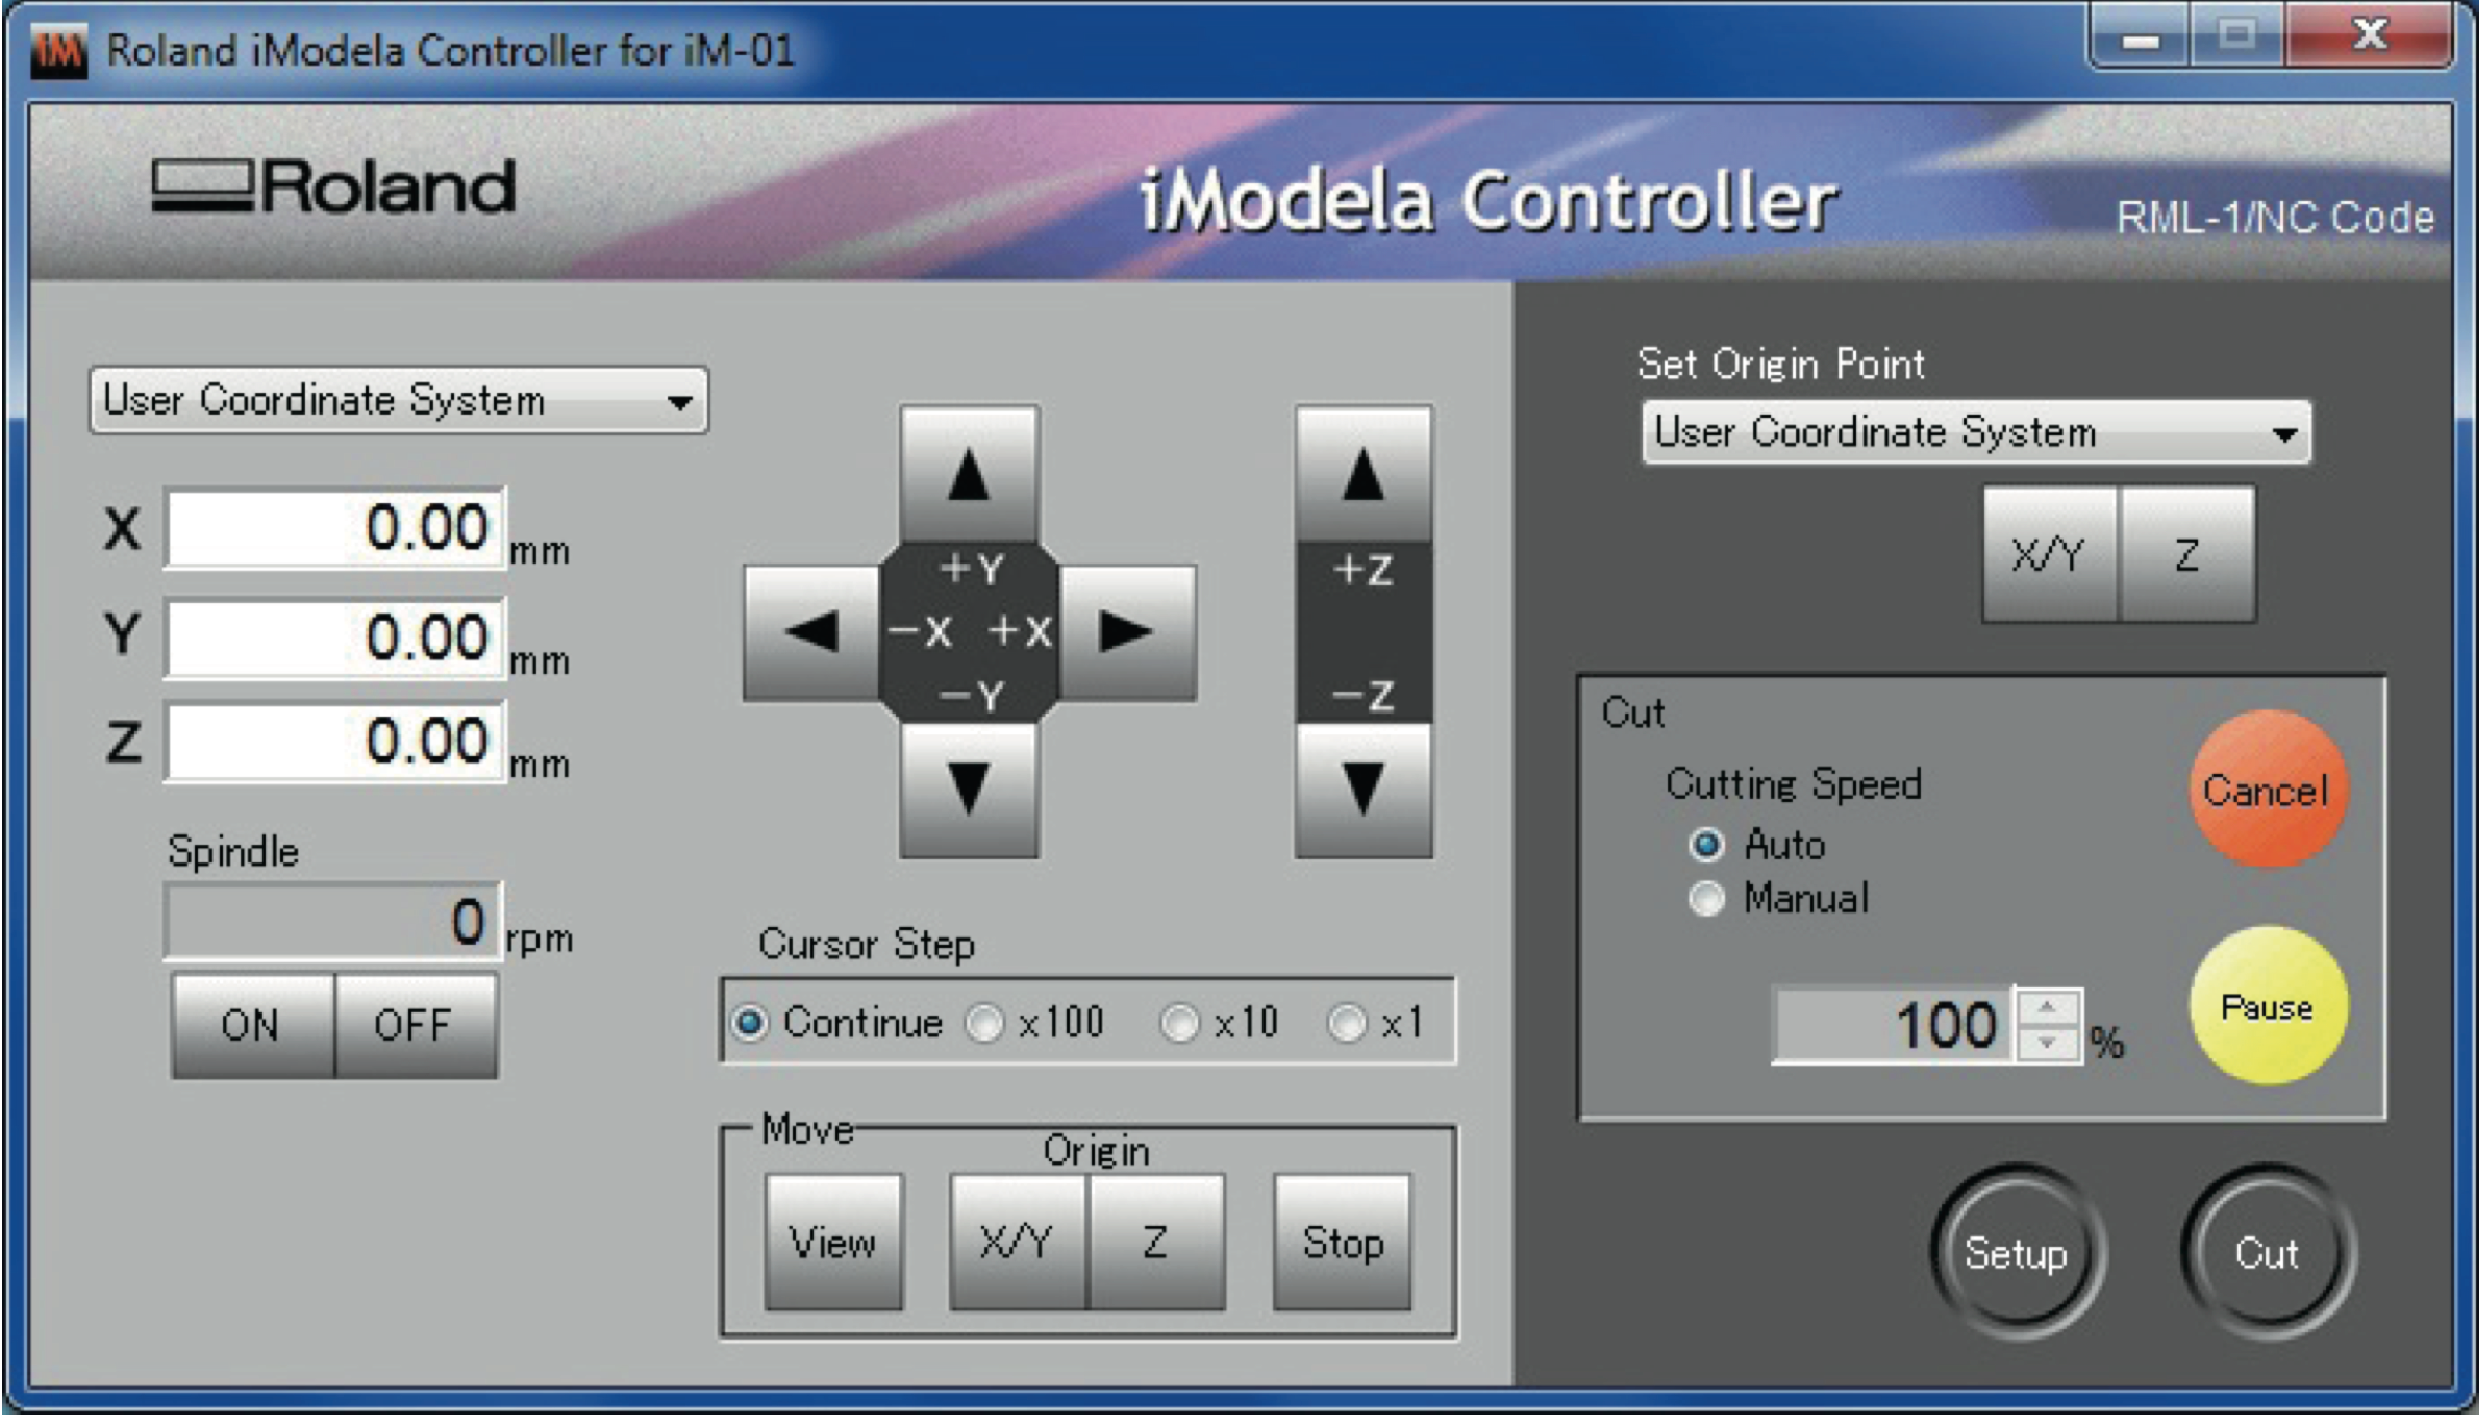
\includegraphics[width=0.8\textwidth]{img/controller}};
    \circled{10}{5}{\textbf{1}};
    \circled{11}{3}{\textbf{2}};
    \circled{0.5}{2}{\textbf{3}};
    \circled{4}{1}{\textbf{4}};
    \circled{3}{5}{\textbf{5}};
    \circled{6.5}{3.5}{\textbf{6}};
\end{tikzpicture}
\vspace{1cm}
\begin{enumerate}[label=\protect\tikzcircled{\arabic*}]
\item Einstellen des XY- und Z-Nullpunktes
\item Automatische oder manuelle Geschwindigkeitseinstellung
\item Spindel an- und ausschalten
\item Fräskopf bewegen
\item aktuelle Koordinaten (immer \emph{User Coordinate System} auswählen)
\item Fräskopf manuell verfahren, mit verschiedenen Schritten oder kontinuierlich
\end{enumerate}
\end{center}

\subsection{Material einlegen}
\begin{itemize}
	\item Das Material wird mit doppelseitigem Klebeband auf einer Opferplatte (z.B. aus Holz) befestigt.
	\item Die Opferplatte wird ebenfalls mit doppelseitigem Klebeband auf dem Frässchlitten befestigt.
	\item Sowohl die Opferplatte, als auch das Material dürfen die Größe 86mm x 55mm (XY-Richtung) nicht überschreiten.
	\item Opferplatte und Material dürfen zusammen die Höhe 26mm  (Z-Richtung) nicht überschreiten.
	\item Um besser an den Frässchlitten zu kommen kann man die Maschine aufklappen (siehe \ref{aufklappen})
	\item \textbf{Wichtig:} es dürfen nur geeignete Materialien gefräst werden. Leitfähige Materialien sind nicht erlaubt. Im Zweifelsfall frage einen Betreuer! 
\end{itemize}

\subsection{Ursprung einstellen}
Der Ursprung deines Objektes sollte sich immer (von vorne gesehen) vorne links an der Oberfläche befinden (roter Punkt). 
\begin{center}
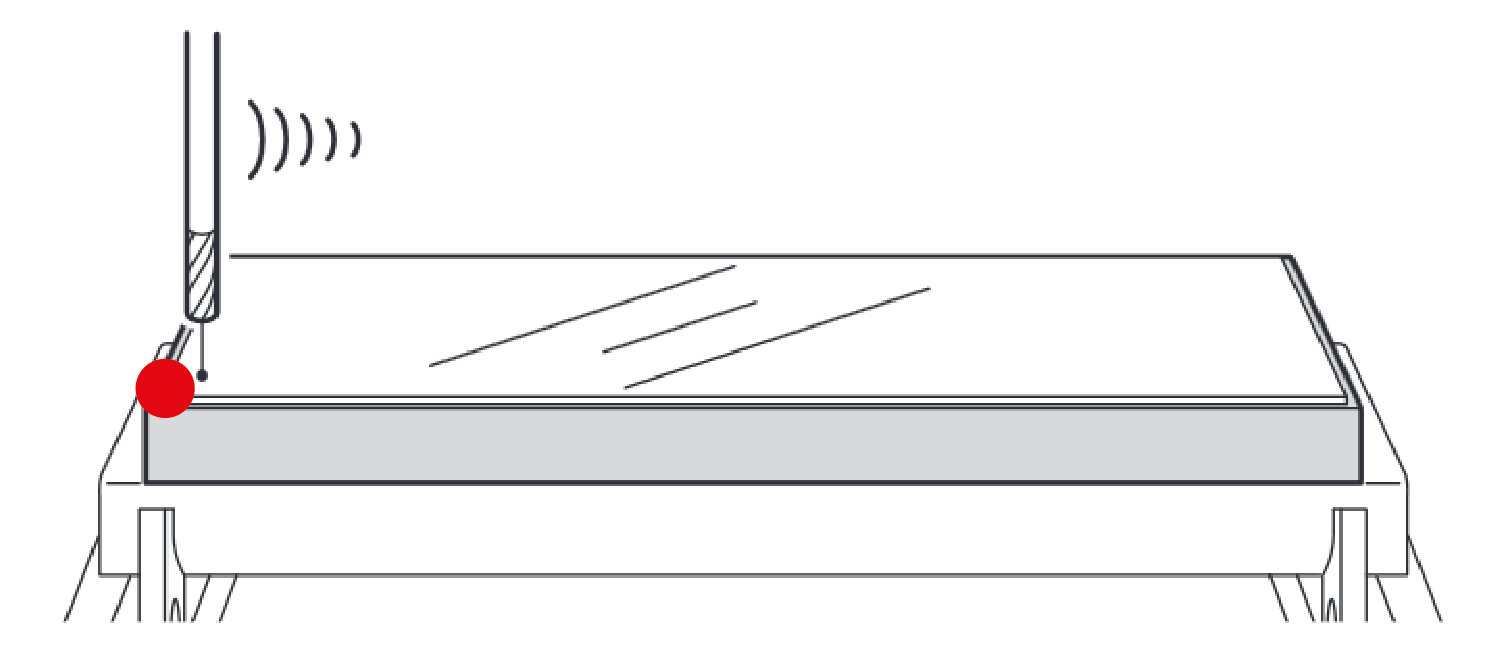
\includegraphics[width=0.7\textwidth]{img/nullpunkt}
\end{center}
Bevor du mit dem Fräsen beginnen kannst musst du den Ursprung auf diesen Punkt deines Materials setzen. Fahre dazu den Fräskopf an diese Stelle (siehe \ref{verfahren}) und setzte den Ursprung in XY- und Z-Richtung. \todo{Bild von Controller} Für bessere Sicht kannst du das Top Cover abnehmen.
\begin{center}
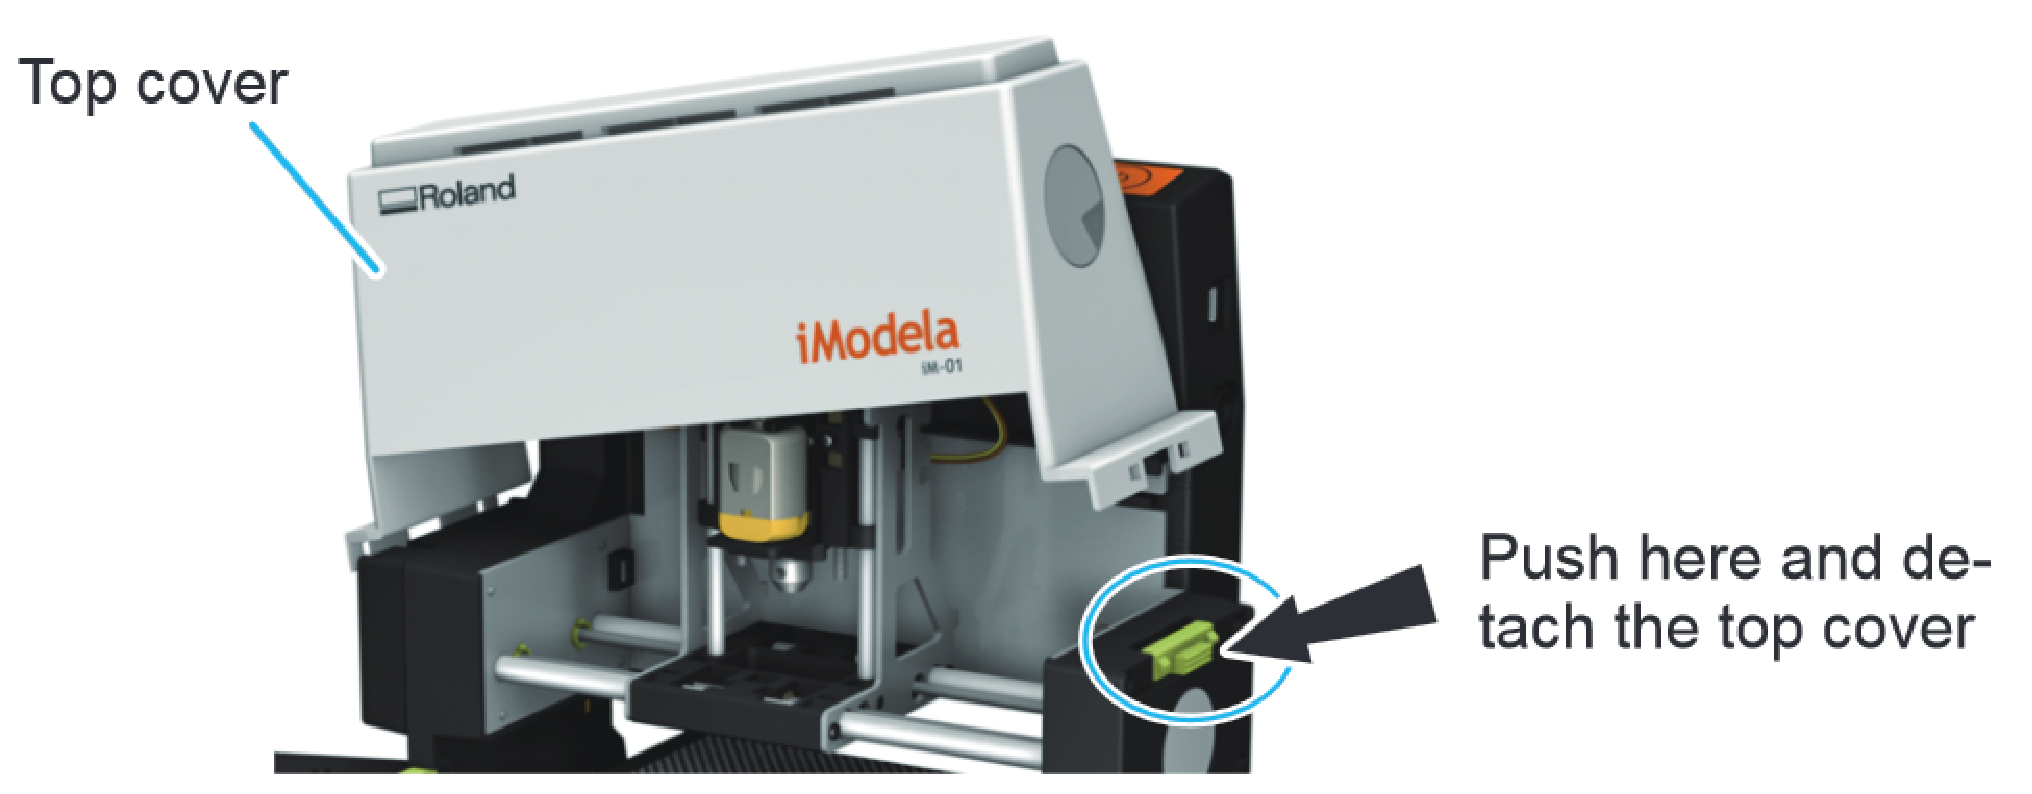
\includegraphics[width=0.7\textwidth]{img/topcover}
\end{center}

\subsection{Werkzeugwechsel}
\todo{...}

\section{Job starten und überwachen}
\todo{...}

\section{Für Betreuer}
\begin{itemize}
	\item Regelmäßiges Fetten! (nach 50 Stunden)
	\item Drehzeit des Spindelmotors: im \emph{iModela Controller} auf den Icon oben links, dann auf \emph{Maintenance}, Tab \emph{Spindle} \todo{englisch oder deutsch?}
	\item Anleitungen für Wartung und Teiletausch in \texttt{Dateifreigabe/1\_fablab/iModela/iModela User Manual}
\end{itemize}

\ccLicense{fraese-imodela-einweisung}{Einweisung Fräse iModela}

\end{document}
